%%%%%%%%%%%%%%%%%%%%%%%%%%%%%%%%%%%%%%%%%%%%%%%%%%%%%%%%%%%%%%%%%%%%
%% I, the copyright holder of this work, release this work into the
%% public domain. This applies worldwide. In some countries this may
%% not be legally possible; if so: I grant anyone the right to use
%% this work for any purpose, without any conditions, unless such
%% conditions are required by law.
%%%%%%%%%%%%%%%%%%%%%%%%%%%%%%%%%%%%%%%%%%%%%%%%%%%%%%%%%%%%%%%%%%%%

\documentclass[
  digital,     %% The `digital` option enables the default options for the
               %% digital version of a document. Replace with `printed`
               %% to enable the default options for the printed version
               %% of a document.
%%  color,       %% Uncomment these lines (by removing the %% at the
%%               %% beginning) to use color in the printed version of your
%%               %% document
  oneside,     %% The `oneside` option enables one-sided typesetting,
               %% which is preferred if you are only going to submit a
               %% digital version of your thesis. Replace with `twoside`
               %% for double-sided typesetting if you are planning to
               %% also print your thesis. For double-sided typesetting,
               %% use at least 120 g/m² paper to prevent show-through.
  nosansbold,  %% The `nosansbold` option prevents the use of the
               %% sans-serif type face for bold text. Replace with
               %% `sansbold` to use sans-serif type face for bold text.
  nocolorbold, %% The `nocolorbold` option disables the usage of the
               %% blue color for bold text, instead using black. Replace
               %% with `colorbold` to use blue for bold text.
  lof,         %% The `lof` option prints the List of Figures. Replace
               %% with `nolof` to hide the List of Figures.
  lot,         %% The `lot` option prints the List of Tables. Replace
               %% with `nolot` to hide the List of Tables.
]{fithesis4}
%% The following section sets up the locales used in the thesis.
\usepackage[resetfonts]{cmap} %% We need to load the T2A font encoding
\usepackage[T1,T2A]{fontenc}  %% to use the Cyrillic fonts with Russian texts.
\usepackage[
  main=english, %% By using `czech` or `slovak` as the main locale
                %% instead of `english`, you can typeset the thesis
                %% in either Czech or Slovak, respectively.
  english, german, czech, slovak %% The additional keys allow
]{babel}        %% foreign texts to be typeset as follows:
%%
%%   \begin{otherlanguage}{german}  ... \end{otherlanguage}
%%   \begin{otherlanguage}{czech}   ... \end{otherlanguage}
%%   \begin{otherlanguage}{slovak}  ... \end{otherlanguage}
%%
%%
%% The following section sets up the metadata of the thesis.
\thesissetup{
    date        = \the\year/\the\month/\the\day,
    university  = mu,
    faculty     = fi,
    type        = mgr,
    department  = Department of Machine Learning and Data Processing,
    author      = Bruno Petrus,
    gender      = m,
    advisor     = {Prof. RNDr. John Smith, CSc.},
    title       = {Segmentation of tunneling nanotubes},
    TeXtitle    = {The Proof of $\mathsf{P}=\mathsf{NP}$},
    keywords    = {keyword1, keyword2, ...},
    TeXkeywords = {keyword1, keyword2, \ldots},
    abstract    = {%
      This is the abstract of my thesis, which can

      span multiple paragraphs.
    },
    thanks      = {%
      These are the acknowledgements for my thesis, which can

      span multiple paragraphs.
    },
    bib         = biblio.bib,
    %% Remove the following line to use the JVS 2018 faculty logo.
    facultyLogo = fithesis-fi,
}
\usepackage{makeidx}      %% The `makeidx` package contains
\makeindex                %% helper commands for index typesetting.
%% These additional packages are used within the document:
\usepackage{paralist} %% Compact list environments
\usepackage{amsmath}  %% Mathematics
\usepackage{amsthm}
\usepackage{amsfonts}
\usepackage{url}      %% Hyperlinks
\usepackage{markdown} %% Lightweight markup
\usepackage{listings} %% Source code highlighting
\lstset{
  basicstyle      = \ttfamily,
  identifierstyle = \color{black},
  keywordstyle    = \color{blue},
  keywordstyle    = {[2]\color{cyan}},
  keywordstyle    = {[3]\color{olive}},
  stringstyle     = \color{teal},
  commentstyle    = \itshape\color{magenta},
  breaklines      = true,
}
\usepackage{floatrow} %% Putting captions above tables
\floatsetup[table]{capposition=top}
\usepackage[babel]{csquotes} %% Context-sensitive quotation marks
\begin{document}
%% The \chapter* command can be used to produce unnumbered chapters:
\chapter*{Introduction}
%% Unlike \chapter, \chapter* does not update the headings and does not
%% enter the chapter to the table of contents. I we want correct
%% headings and a table of contents entry, we must add them manually:
\markright{\textsc{Introduction}}
\addcontentsline{toc}{chapter}{Introduction}

Theses are rumoured to be \enquote{the capstones of education}, so
I decided to write one of my own. If all goes well, I will soon
have a diploma under my belt. Wish me luck!

\chapter{Data}

Our work begun when the Estonian partners send us the four different datasets of
the wanted to study phenomena. To study the effects of tunneling nanotubes which
are these thin, long and often time curved structures, they deciced to use wings
of fly larvae. A schematic can be viewed in Figure [TODO]. This is quite
interesting sample as it generaly has, as can be seen in Figure [TODO] and
[TODO] two distinct layers of cells, between which a vertical pillar like
structures are visible. These structures are what we will refer to in this work
as pillars for simplicity. These belong to the [FINISH] part of the wings. How
such data can be acquired and for more information of the process I recommend
looking into the \parencite{Tran2024Programmed} paper.

\section{Acquired Datasets}

The data was captured using fluorescence microscopy. [TODO simple explanation]
and four distinct datasets were acquired. Three of these datasets were captured
with two different channels, larger volume and smaller spatial resolution. All
the datasets are actually part of a time series as it is of quite interest in
looking at the temporal properties of the biological phenomena i.e. do tunnels
stay for multiple steps or are they short-lived? Does their properties change in
time? But that was not the main point of our current research.

The last dataset contains just one channel. The fluorescent dye was selected to
highligh both the pillars and the tunnels as can be seen in Figure [TODO]. As we
can see unlike the previous datasets this was capture at much higher spatial
resolution; therefore, we can see that the dye react mostly in the cell membrane
and they appear hollow. Moreover, the tunnels are much more visible compared to
the previous three datasets, but it only contains a single channel now.

As said before the data was captured by our Estonian partners at [TODO], to
further propel the research they promised us to annotate the three large
datasets, but after several months no labels were given which complicated the
research and work. Hence, we approached our collegues at [TODO what fac.] and
they were kind enough to help us.

\begin{figure}
    \begin{center}
        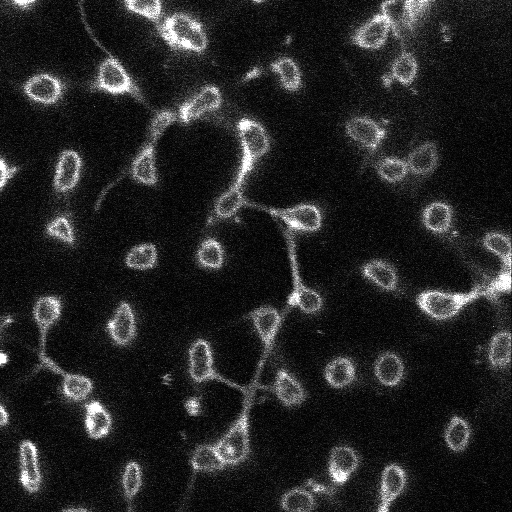
\includegraphics[width=0.6\linewidth]{resources/t017z0_saturated1percent.png}
    \end{center}
    \caption{First slice of the data at time step 17, after the biologist
    preprocessing pipeline}.
    \label{fig:biologistpreprocessing}
\end{figure}

\section{Labelling and preprocessing}

The biologist created a protocol which they followed by annotating the samples.
They decided to preprocess the data by converting the images from 16bit
grayscale image into 8bit grayscale images, then a 1\%-percentile stretch was
applied to further enhance the images. The result of the preprocessing is
visible in Figure \ref{fig:biologistpreprocessing}. As can be seen on the figure,
this makes the tunnels easier to see at the cost making noise more visible.

After the preprocessing is done, the protocol states that picking random time
slots at least 100 instances of tunnels must be annotated, and each frame has to
be fully annotated. According to this protocol the biologists picked two time
steps --- the 0th and 17th step --- and gave us uniquelly labeled data, an
example can be seen in Figure [TODO] also with an overlay of the labeles, over
the data. In this case however, I removed the unique labels for better
visualisation.

The labels were manually checked by me and a single case of label duplicity was
found at time step [TODO], where two different tunnels were assigned the same id
of 33. I manually fixed this and assigned a new unique label. In Figure [TODO] a
maximum projection across the depth can be seen visualising the two problematic
tunnels.

\chapter{Architectures}
This chapter deals with what neural network architectures were used in
developing the solution.

\section{Preliminary research}
We began by researching similar papers dealing with segmenting nanotubular
structures. Two promising papers we found are ..[TODO]. In

\parencite{Hodneland2006Automated} the researchers are similar to use dealing
with tunnels between cells, but in their case the tunnels form a long straight
lines. In the paper they describe a multistep algorithm which takes employ two
channels, one is for segmenting cell borders and tunnels, while in the other
channel the cells inside are much more visible, hence, this can be used to
better separate cells and tunnel.

As our data has different modality, this approach could not be used. They also
assume that the tunnels are straight which is not true in our case.
The other paper which specificaly mentiones tunneling nanotubes is
\parencite{Ceran2022TNTdetect}. This paper provides consists of three parts.
They describe how to improve the labels and make it easier 

\section{U-Net}

In 2015 a seminal paper by Rossenberger et al. \parencite{Ronneberger2015} was
published dealing with semantic segmentation of medicine data. The paper
achieved impressive results with very limited dataset. The neural network
architecture is called U-Net and has been behind many models later to come.
[TODO citation]

\begin{figure}
    \begin{center}
        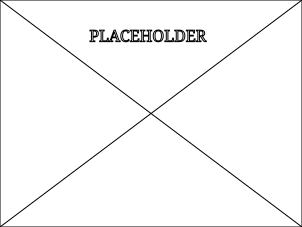
\includegraphics[width=0.6\linewidth]{resources/placeholder.png}
    \end{center}
    \caption{A UNet architecure diagram}.
    \label{fig:unetdiagram}
\end{figure}

The key architectural part of the U-Net lays in the introduction of transposed
convolution layers which upsample the result of the encoder. This is placed
after what traditionally like in the neck in VGGNet [TODO citation] was followed
by a classification head now follows the decoder. A diagram can be seen in
Figure \ref{fig:unetdiagram}. As can be seen in the figure, on input it takes an
image and it is followed by a horizontal block formed of two convolutions,
followed by a max pool operation which downsamples the image by a factor of 2.
After this is done numerous times, which depends on the depth of the network set
by the user, additional convolution is applied. The results of the neural
network before the downsample operation is taken is also saved. After the neck
part a series of upsampling operations take place. This is achieved using a
transposed convolution operation and the weights are learned automatically by
the network. Note that other possibilities, like using interpolation in [TODO
citation] was not researched in this work. This upsampling operation doubles the
spatial resolution at the cost of halving the number of channels. Each time such
operation takes place the result of relevant encoder layer is concatonated,
followed by two additional convolutions. Finally we do a final convolution
operation to ouput the right amiunt of classes, which in our case is equal to
two (tunnel or BG/pillar).

The two main reasons for choosing this architecture compared to other was that
the U-Net architecure is well estabilished, widely used, achieves good
performance [TODO citation], but mainly due its nice property that Rossenberger
et al. \parencite{Ronneberger2015} demonstrated that you do not need a huge
dataset to teach the neural network. As our data is quite limited in terms of
size this is a very usefull feature.

The Figure \ref{fig:unetdiagram} is visualising how the UNet architecure can be
used to train a 2D model, but there is not reason why we could not use 3D
versions of convolution, maxpool and transposed upconvolution. 

\subsection{Anisotropic U-Net}

In machine learning it is often tried to increase the model depth to improve the
perfomance of the neural network. This is of course not true universaly as this
can make the network harder to train can cause the network to overtrain [TODO
citation needed]. Since our data is heavily anisotropic we are limited in how
much we can downsample in the z direction, as we have only 7 voxel inside the z
dimension, it is possible to downsample just two times before reaching depth
equal to 2. Moreover, it would probably be reasonable to assert that compressing
all the depth information into a single channel is asking the neural network to
do a lot of work compressing the info.

This problem motivated us to create a new version of the U-Net which uses
anisotropic kernels instead of isotropic kernels for both convolution and the
maxpool operation.

\begin{figure}
    \begin{center}
        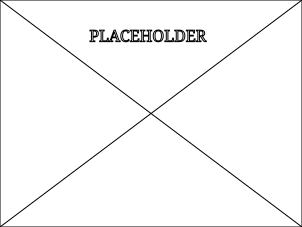
\includegraphics[width=0.6\linewidth]{resources/placeholder.png}
    \end{center}
    \caption{Visualisation of 3D convolution and maxpool operation}.
    \label{fig:visanisooperations}
\end{figure}

As is ilustrated in Figure \ref{fig:visanisooperations} a 3D convolution
uses a 3D kernel to look into a 3D part of the input. By appriopriately padding
the output, we can keep the same dimension in the z axis. Moreover, to prevent
early downsampling in the z dimension we can use anisotropic versions of these
operators. Instead of downsampling by a factor of 2 in all directions, we can
ignore downsampling in the z dimension by setting the kernel size in that
direction equal to 1 [TODO or 0?].

\section{The CSAM module}

This section talks about the channel and spatial attention module (further
refered to as the CSAM) mentioned in the CS-Net paper \parencite{Mou2021}. In
this paper the author tried to improve the performance of UNet architecture by
incorporating attention into the model. This was motivated by using the
architecture for segmenting blood vessels and related biological features and
seeing that one of the problems which was often encoutnered is the fact that
these network had trouble connecting faint blood vessels leading to a
connectivity issues. The attention models helps with connecting them together.

Even though we are not dealing with vessels in our case, the tunnels do visually
resemble some curvilinear structures. We also encountered some of these issues
with connectivity, and as such this might also alleviate the our problems [TODO
reference].

\begin{figure}
    \begin{center}
        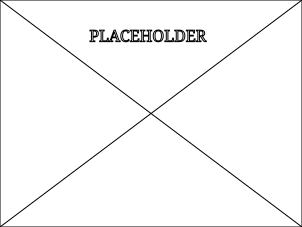
\includegraphics[width=0.6\linewidth]{resources/placeholder.png}
    \end{center}
    \caption{The CSAM module from Paper [TODO CITE]}.
    \label{fig:csammodule}
\end{figure}

The Figure \ref{fig:csammodule} by \parencite{Mou2021} explain the working
principle behind the CSAM module. It is formed of two paths, the spatial
attention block SB and the channel attention block CAB. One is designed to help
the network find tubular structures inside the spatial direction while the other
is used for helping the network learn inter-channel dependency.

\subsection*{SAB}
The design is motivated by the detection of tubular structures such as blood
vessels in retina images. The detection of such features might require
contextual information rather than purely local information. This lead the
author to use anisotropic kernels 

\subsection*{CAB}
The design ...



\section{Squeeze and excitation block}
In Paper \parencite{Hu2018} researchers demonstrated how a simple small block
can be inserted inside deep neural networks to improve their performance accross
various datasets and tasks. The researchers postulate that this block helps the
network learn inter channel dependecies [TODO where in paper].

\begin{figure}
    \begin{center}
        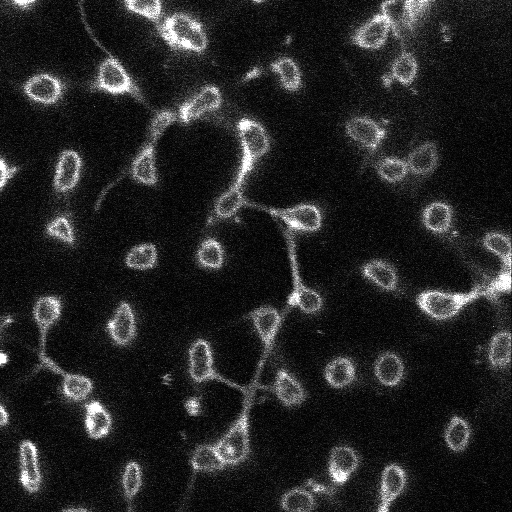
\includegraphics[width=0.6\linewidth]{resources/t017z0_saturated1percent.png}
    \end{center}
    \caption{Squeeze and exciation block from Paper \parencite{Hu2018}}
    \label{fig:se_diagram}
\end{figure}

The general principle of a squeeze and excitation block is illustrated in Figure
\ref{fig:se_diagram}. The main idea is that we let the network learn
significance of each channel. This is technically done by multiplying the data
$U$ by a number from 0 to 1 in each channel separately.

The squeeze and excitation block consists of four operations: truncate, squeeze,
excitation, and scaling. The truncate operation shown as $F_{TR}$ is a general
convolution operator, which reduces the dimension. This step is not crucial in
the scheme, but it is mainly to illustrate the point, that SE block is usually
built upon some operation. More importantnly, the transdormed data is taken and
run through a squeeze operation, which basically does some global operation in the
whole channel. After that, the excitation operation comes. This operation was
designed to have the following properties: they wanted to create a flexible
operation --- meaning an operation capable of learning non-linear dependecies
--- and they wanted it to be non-mutually exclusive between channels. This is
done by applying two convolutions followed by ReLU and sigmoid respectively.
Note that the first convolution produces output with less than the original
number of channels and the ratio is called the reduction factor. Finally the
last convolution expands the number of channels to the original size. The
comvination of squeeze and excitation allows the network to learn how to weight
each channel (the scale operation mentioned above) by considering multiple
channels.

\begin{figure}
    \begin{center}
        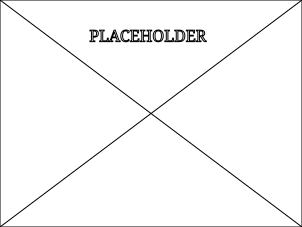
\includegraphics[width=0.6\linewidth]{resources/placeholder.png}
    \end{center}
    \caption{Placement of SE blocks inside the U-Net by \parencite{Rundo2019}}
    \label{fig:se_unet}
\end{figure}

Another issue is where to put this block, as I already mentioned the truncate
operation, the authors suggest placing it after applying convolution, they also
suggest placement in the Inception and ResNet blocks [TODO citation?]; however,
placement inside a UNet architecture is not mentioned. After further
considerations [TOOD what options] the blocks were placed according to Paper
\parencite{Rundo2019} after every step in the decoder and after each upsampling
step as is shown in Figure \ref{fig:se_unet}.

\chapter{Processing data}
splitting and stuff

\chapter{Training}
how the neural networks were trained.

\chapter{Evaluation}
how we evaluate the networks

\chapter{Ablation studies}

\chapter{Implementation}

\section{Used technologies}
Python, mlflow, Bash, uv

\section{Use case modelling and expected usage}

\chapter{Discussion}
what to do next

\end{document}
